
\section{Protocol}

In this section we describe the Lakat protocol. We start with a high-level overview of the protocol and then go into the details of the individual components. Lakat is a shared key-value database of branches and data buckets together with a peer-to-peer protocol that governs the modification of this database. The modifications happen through submits to branches. The protocol needs to cover five functions: 1) Define a mechanism to construct new contributions \footnote{This is called block proposal for blockchains. Examples include proof-of-work or proof-of-stake}. 2) Broadcast information about requests and new branch modifications through the network. 3) Check the validity of the branch modification. 4) Define a strategy to finalize the state of a branch. 5) Incentivize contributors to propose modifications. 

Lakat proposes a local consensus mechanism that relies on the notion of branch contributors. In principle Lakat could be used with various consensus mechanisms at branch level, such as proof-of-work or proof-of-stake. However, we propose a new one that we consider more suitable for academic publishing. This mechanism combines three concepts: 1) The distinction between \textit{feature and production} branches 2) A \textit{proof-of-review} mechanism that is used to propose new states of the production branch 3) A finality mechanism that is used to finalize the head of a branch, which we call \textit{lignification}. The incentive mechanism is not built into Lakat, but may be added on top of it through the token handling at the level of the branch. Even in the current publishing business the incentives are outsourced to reputation, job promises and in some cases mere scientific curiousity. If anything, there is an anti-incentive to publish. In the following we describe the individual components of the protocol in detail.

\subsection{Networking}
\label{ssc:networking}

On of Lakat's components is an asynchronous networking protocol, where peers can enter and leave at any time. The state of the individual processes of each peer is communicated and updated through a gossip protocol. The gossip protocol is used to broadcast requests and branch modifications to the network. We use the Kademlia DHT for this purpose. In Lakat the gossiping network is used to store the information state of the individual peers. This includes the branch requests (see Subsection \ref{ssc:branchrequests}) and the high level information the states of the branches that this peer keeps track of. This high level information consists of the branchId, the parentBranch, the branchConfig (branchType, acceptConflicts, acceptedProofs, consensusRoot), the stableHead (parent submit, submitMessage, trieRoot, submitTrace), the sprouts, sproutSelection, branchToken and timestamp (see Subsection \ref{ssc:branch}). What about the bulk of the data, namely the data trie with all the data buckets and their respective interaction information, and the trace of the stableHead? That is optionally outsourced to other protocols. The protocols are then part of the multihash. They could include e.g. ipfs, filecoin, urbit\footnote{We also consider building on top of the Urbit OS using linedb\cite{linedb} as a key-value storage and networking solution} or if that peer chooses to do so, it could also store the data locally in the hash table. In Kademlia proximity of data is measured in proximity of the content identifier of the data. In future releases of Lakat we propose to tweek the proximity such that data stored on the same branch is close to each other. We are planning to use the libp2p library as a basis of the networking protocol. It is a modular networking stack that uses Kademlia.  


\subsection{Local Consensus}
\label{ssc:localconsensus}

Who decides which content will be added to a branch? In lakat there is no global notion of what counts as science and what does not. There is only a local notion, the detailment of which is the subject of this section. A global consensus mechanism seems to be a good fit for a ledger that keeps track of values that are or ought to be globally agreed upon, i.e. for values that exist qua their global agreement. In contrast to money transactions, the global scope seems ill-fitted for the publication of research content. In our view this requires a local form of consensus. In the context of Lakat, the scope of the locality is at the branch-level. 

What does a branch-level scope mean? This means that the scope is constrained to the \textit{contributors} of a branch. Every branch has a history of submits and is \textit{rooted} in some parent branch or is itself a \textit{seedling} (See Subsection \ref{ssc:branch} regarding roots and seedlings). In either case there is a set of contributors to every branch between its root and the current head. Any actor, human or AI, who can prove to have contributed content in any of the branch's submits counts as a contributor (See Subsection \ref{ssc:contributor}). 

Branch contributors form the basis of the consensus mechanism. We entrench this deep into the protocol by allowing only branch contributors to make changes to the branch that they are contributing to. This design choice also keeps potential attackers from pushing unwanted content to a branch. Lakat does not make statements about what counts as science and what not. What counts as a legitimate scientific contribution purely emerges through the local consensus. One contribution that is viewed as being unfounded or unscientific for one branch might be viewed the opposite on another branch. In some sense this reflects a Feyerabendian approach \cite{}. It gives space for pluralism and allows for the organic selection of branches with possibly differing criteria on what counts as valid output. There is, however, a convergence in accepted method and output expected to emerge within a branch and also in branches that are close to each other. Branches that are close have branched off recently and possibly disagree more on technical grounds than on methodic grounds or they are simply feature branches that are to be merged back into the main branch soon. There is an overall incentive to merge branches, derived from the persistence of the data and the value of the token (see Subsection \ref{ssc:incentive} for possible incentive structures). 

The local consensus paradigm is governing amendments to branches, both to twigs and to proper branches. Sprouts on the other hand are just auxiliary objects that cannot be modified directly and are thus not amenable to a consensus mechanism. The consensus paradigm for twigs simply states that any branch contributor can push submits to the twig whereas merging into a twig requires a certain fraction of contributors to agree (See Subsection \ref{ssc:twigs} for twigs and Subsection \ref{ssc:twiglocalconsensus} for consensus on twigs). For proper branches the local consensus takes on a different form. It is divided into proof of review (See Subsection \ref{ssc:por}), broadcasting and lignification (See Subsection \ref{ssc:lignification}).

\subsection{Feature Branches}
\label{ssc:twiglocalconsensus}

Twigs are meant to be used for rather quick iteration. They behave like feature branches. Here is an example where twigs are expected to be used: If a contributor, human or AI, would like to add content to a target branch, say an article or some modifications or both, it creates a feature branch rooted in the target branch which subsequently goes through the proof-of-review consensus mechanism (see Subsection \ref{ssc:por}). Typically the number of content contributors on a twig will be low. Maybe a single author or a small group of authors, as it is the case for article publications. In order to not compromise the momentum and the quick iteration both content contributors and review contributors (if there are any) can push to the branch directly. Merges can also be pushed, but require a fraction of approvals of the content contributors. The fraction is determined in the config of the twig. 

\subsection{Proof of Review (PoR)}
\label{ssc:por}

Before a branch can be merged into a proper branch it needs to undergo a review. Table \ref{tab:reviewProcess} summarizes the steps.
% % We describe this process keeping to the notation of \textit{belt} as the branch that seeks to be merged and \textit{core} as the target of the merge (see Subsection \ref{ssc:branch} for the terms core and belt).
To start the review process an \textit{issuing branch} creates a pull request from a \textit{requesting branch} to a \textit{target branch}. The pull request is a submit with two properties: First it contains a newly created context data bucket, called the \textit{review container}, that will hold all the forthcoming information of the review. The submit may of course contain other buckets besides that. Second, it leaves a trace of the information about the pull request in the pullRequests entry of the \textit{submitTrace}, namely pointers to the review container, to the target branch and the requesting branch. In most cases the review happens on a twig, which acts as a feature branch. There the issuing branch and the requesting branch are identical, because the twig requests for itself to be pulled into the target branch. However, the requesting branch may also act as a proxy requester. This is the case when a proper branch rather than a twig seeks to be merged into a target branch. Since this intention itself must pass through the consensus rule of that proper branch, one would have to create a twig and include therein the proxy pull request. Once that twig is successfully merged into the actual requesting branch by passing the consensus, the review process can begin on that proper branch for it be mergeable into the target branch. We call a pull request \textit{mature} once it is included in the requesting branch. In the most common scenario where the issuing and requesting branch coincide maturity is immediate. 
% In the ensuing merging process the requesting branch becomes the belt and the target branch becomes the core.}
Once a pull request becomes mature a message will be send to the target branch  where its contributors are invited to review the requesting branch. The message is simply a reference to the pull request sent to the pullRequests channel of the target's \textit{branchRequests} (see Subsection \ref{ssc:mempool} for branch requests).
Any content contributor of the target branch who is not also contributing to the requesting branch can then become a \textit{review contributor} of the requesting branch. They must first publish a review commitment on the requesting branch. This makes them official contributors to that branch. It also helps to gauge general reviewers engangement prior to the actual review. This is helpful both for those who seek to merge and those who seek to review. It also increases accountability of the committing reviewer. Failing to supply a review after a commitment could be penalized via the social engagement (see Subsection \ref{ssc:socialrefs}).  
Committers publish their commitment in the reviewsTrace of the submitTrace. They cannot submit reviews without a prior commitment. Also, the identity of the reviewer is not public in the sense that the commitment solely contains a zero-knowledge proof that the reviewer is a contributer to the target branch (see Subsection \ref{ssc:contributors}).
Of course the reviewer may decide to reveal their identity and this may or may not be in line with the configuration of the target branch.

Reviewers then push review submits to the requesting branch. The submits just contain a proof of contributorship in the target branch. A review submit consists of the following: A bucket with a review, called a \textit{review item}. This bucket should reference all the data buckets that it has reviewed. In the respective interaction data (see Subsection \ref{ssc:branch}) of all those reviewed buckets a reference to the review item is stored within the reviews entry. Finally the review item gets referenced in the review container of the pull request. Updating the review bucket, as with any bucket update, consists of creating a new review bucket that points to the old one through the parent entry\footnote{In future versions of Lakat we wish to move to updates via deltas.}. The branchConfig of the target branch specifies the pre-requisites for a merge. This consists of the minimum number of reviewers, a rule for acceptance and a minimum number of review rounds, which could be one by default. The rule of acceptance could be preset aswell. For instance one could reject requests when a certain fraction of reviewers reject and accept when there are no rejections and specify some rule for the middle ground. Once all the requirements of the target branch are satisfied the branch is ready to be merged. 

How about merging branches that do not seek to be merged? This can be the case when trying to merge the newest developments from a remote branch. This case is in fact already covered by the respective consensus mechanisms of twigs and proper branches. Merging into twigs requires a fraction of content contributors to agree (see Subsection \ref{ssc:twiglocalconsensus}). Merging into proper branches requires a pull request and subsequent reviews, so it is not possible to just merge other un-reviewed branches in the same way that one merges reviewed twigs or reviewed proper branches. Therefore, one would have to create a twig that merges the remote branch as a feature. It then requests to be merged und the merge undergoes a review. \remark{clarify}



\begin{table}
  \begin{tabular}{|p{0.025\textwidth}|p{0.3\linewidth}|p{0.595\textwidth}|}
  \hline
  \textbf{\#} & \textbf{Step} & \textbf{Description} \\
  \hline\hline
  1 & Create pull request & The issuing branch creates a request for the requesting branch (in most cases identical) to be merged into the target branch. A review container is created. \\
  2 & Maturity of the pull request & The pull request is included in the requesting branch (in most cases immediate)\\
  3 & Commitment & A content contributor of the target branch publishes a review commitment to the requesting branch. That makes them review contributors of the requesting branch.\\
  4 & Review & The review contributors create review submits that are referenced in the review bucket.\\
  5 & Completion & The number of review cycles and the coverage of the review meets the criteria of the target's branchConfig. The branch may be merged into the target.\\
 \hline
  \end{tabular}

  \caption{Overview of the Proof--of--Review (PoR) process}
 \label{tab:reviewProcess}
\end{table}

\subsection{Broadcasting and Lignification}
\label{ssc:lignification}

How are the reviewed pull requests bundled up and sequenced into a single proper branch? Why is the process important? How is the required attention bandwidth for this proess kept to a minimum? In order to explain the Lakat answer to this question we first contrast it to the case of blockchains: There transactions are bundled into blocks. They are then broadcasted across the network of nodes. When different blocks with the same parent are broadcasted, there will be conflicting versions of the blockchain state, which for a single source of truth is undesirable. In ethererum prior to the transition from the proof-of-work to the proof-of-stake these alternative versions were called ommers and were mostly the result of latency in the broadcasting, but of course also attacks or client-software issues. To make sure that a transaction has irrevocably been added into the blockchain one would have to wait for a few block confirmations. 

In Lakat we solve the issue through a process that we call \textit{lignification}. The idea is that amongst the potentially plentiful and conflicting versions of the new branch state eventually a new head will be chosen. This head is then called the stable head. The versions are stored as short-lived branches, called sprouts. The \textit{sprouts} entry of the branch points to them. Why is the process of choosing a successor to the stable head important? Here is an explanation: The branch is an object that is kept alive by an ecosystem of contributors. It could get hijacked by a group of bad actors who became branch contributors through a mal-reviewed pull-request. In principle, if this happened, the contributors that disagreed with this malicious onboarding could bail out by creating a new branch. However, this new branch would have to grow the reputation of its contributors anew, seek new storage providers, have a new branch token and would generally have to start from scratch. It might not even be an attack, but a disagreement in the community that leads to a branching.
Even though the process of finding a new stable head constitutes an important security measure for the branch, it should not create an overload of attention demanded from the target branch contributors. In most cases there will be no action required. But it is precisely those rare cases, where such a security measure becomes valuable. So one of the requirements for this process is that the branch production continues unambiguously when there is no interference from the community of contributors. In the following we introduce the process of broadcasting and lignification in more detail.

\subsubsection*{Broadcasting}

Henceforth we refer to our proper branch as \textit{core}. It functions as a production branch. Every proposed new merge submit could either become the stable head of core or become the first submit of a new (disagreeing) branch that is rooted in core. We refer to any of those new branches collectively as the \textit{peri} branch. Not that the \textit{core} branch may also become \textit{peri} for another branch. Merge submits carry in themselves the possibility of becoming the head of a new branch. Therefore we decided to "wrap" them into short-lived proto-branches, namely sprouts, whose respective heads are the merge submits. The process of broadcasting is as follows. A content contributor of core, let's call her Alice, creates a merge submit, which is a special kind of submit (see Subsection \ref{ssc:submit} \remark{ToDo}). This submit is then wrapped into a sprout, which means that the head of the sprout is set to be the merge submit and the content contributors are set to be the union of Alice and all the contributors of the pull-requesting branch. Let's call this sprout \textit{S}. The branch information of the sprout becomes relevant if it eventually turns into a proper branch, a process which is discussed in the lignification part of this Subsection. The parent of the merge submit is the head of a branch \textit{B}, that is either the core or any of the sprouts upstream of the core\footnote{The sprouts entry of a proper branch keeps track of all the upstream sprouts, but depending on the last branch update may also contain outdated sprouts. In order to retrieve all upstream sprouts one may "walk" upstream using the sproutSelection entry, which only contains the immediate offspring sprouts of a given branch.}. Alice chooses \textit{B}, so she decides where to root the new sprout. If she decides to point to a branch that is already pointed at, there will be a conflict. The new sprout \textit{S} -- or rather its branchId -- is then added to the sproutSelection entries of \textit{B} and the sprouts entry of the core (which might coincide with \textit{B}). The new state of core is then broadcasted to all contributors of core. Note that the new state of core might have received more updates than just the modification of the sprouts or sproutsSelection entries. There can also be further modifications resulting from the lignification process (see next part). The changes, i.e. creation, of the sprout branch \textit{S} are also broadcasted to its contributors. 

\subsubsection*{Lignification}

Once a given submit is the new stable head of core or of peri, it cannot be revoked. We say it is \textit{lignified}. The conversion of a previously flexible object into a rigid amendment of a branch has similarities to the process of lignification in botany. 
The decision about the stable head is not made immediately, but there is a period of time where it can still be revoked and deferred. This time is called \textit{lignification time}. As mentioned above, the objects that we make decisions about are not the merge submits themselves, but the sprouts that contain them. If there is only one sprout available after the lignification time, then the decision is clear, namely that the submit contained in that sprout becomes the new stable head of core and no action is required. However, there may be multiple sprout options. In this case, we propose to have a deterministic rule that singles out one sprout and we suggest the possibility of vetoing the default deterministic choice. This minimizes the need to vote each time multiple options arise, but more importantly it reduces the attack vector for people to bring branch growth to a halt by proposing alternate -- yet still reviewed -- merge submits. Vetoing is possible throughout the lignification time. Any branch contributor may register a veto to any of the vying sprouts and therefore against the default sprout. In case that a veto is registered the sprout in question has a chance to provide the next stable head. \remark{how does that work in practice and where is the veto registered and every proposal of new merge submits can also advance the state of the stable head ...}
Once a veto is registered, the content contributors can bring in their votes on the rivaling sprouts. After a period of time, called the \textit{engagement time}, the winning sprout will provide the new stable head and the other sprouts can turn into peripheral proper branches rooted in core. Like with blockchains, the state of Lakat does not change by itself, but only through transactions (See Subsection \ref{ssc:transaction} for transactions). This means that only when a new submit is broadcasted can the state of a branch be updated. Furthermore, a branch may only be updated if it is the target of a transaction. If the transaction is targeting core, then peripheral branches cannot be updated and vice versa. As a consequence those ousted rivalling sprouts do not turn into their own branches immediately, but only once a transaction targets them. Some of them may never turn into proper branches at all. Apart from the lignification time and the optional engagement time there is a time allowing for latency issues in broadcasting, called the \textit{broadcastingBuffer}. This ensures that the timestamped vetos or votes are broadcasted and thus recorded before the stable head is irrevocably fixed.

Due to the time between successive transactions it is quite possible that the state of the core, in particular its stable head, needs to be updated. Maybe the veto time or the voting time between rivalling sprouts has passed or maybe there are no rivalling sprouts and the stable head simply needs to be advanced. The speudo-code in the Lignification Algorithm \ref{alg:lignification} outlines the iterative procedure that advances the stable head on each new transaction. It is worth noting that also the sprouts entry and the sproutSelection entry of core get updated by pruning and replacement respectively.
An illustration of the lignification process is also shown in Figure \ref{fig:bufferbranches}.

In practice the broadcasting and lignification can be automated by a script so that it requires less cognitive bandwidth. The script would choose a content contributor of core at random and broadcast collect all the pull requests that meet the merge-requirements from core, then create one or more merge submits from them, go through the lignification process and broadcast the result. Only in the case when there are disagreements would a manual interference be required.

\begin{algorithm}[h!]
\caption{Lignification -- Advancing the stable head of the branch}
\begin{algorithmic} 
\REQUIRE coreBranch, mergeSubmit, broadcastingBuffer, lignificationTime, engagementTime 
\STATE downstreamBranches $\leftarrow$ branches downstream of coreBranch: [coreBranch, ..., sproutOf(mergeSubmit)]
\STATE referenceBranch $\leftarrow$ coreBranch \comment{/* referenceBranch may later be core or peri(pheral) branch */}
\FOR {i in 1 ... (downstreamBranches.length - 1)  \comment{/* indexing starts at 1 */}}
  \STATE currentBranch $\leftarrow$ downstreamBranches[i]
  \STATE childSprout  $\leftarrow$ downstreamBranches[i + 1]  \comment{/* always exists */}
  \IF {all currentBranch.sprouts are within lignificationTime time (plus broadcastingBuffer)}
    \RETURN
  \ELSE
    \IF {There is a veto against defaultSuccessor(currentBranch) and voting has finished}
      \STATE \comment{/* engagementTime is over (plus lignificationTime plus broadcastingBuffer) */}
      \IF {childSprout does not win the vote}
        \STATE \comment{/* doesn't participate (not defaultSuccessor or not part of a veto) or participates and doesn't win */}
        \STATE childSprout becomes a peripheral branch rooted in referenceBranch.
        \STATE referenceBranch $\leftarrow$ childSprout.
      \ELSE 
        \STATE \comment{/* childSprout wins the vote */}
        \STATE set the stableHead, sproutSelection and sprouts of referenceBranch to those of childSprout
      \ENDIF
      \STATE \comment{/* childSprout may or may not be defaultSuccessor. Both cases are covered. */}
    \ELSIF {There is a veto against defaultSuccessor(currentBranch), but voting has not finished}
      \RETURN
    \ELSE 
      \STATE \comment{/* There is no veto against defaultSuccessor(currentBranch) */}
      \IF {childSprout is defaultSuccessor(currentBranch)}
        \STATE set the stableHead, sproutSelection and sprouts of referenceBranch to those of childSprout
      \ELSE
        \STATE childSprout becomes a peripheral branch rooted in referenceBranch.
        \STATE referenceBranch $\leftarrow$ childSprout.
      \ENDIF
    \ENDIF
    \STATE \comment{/* Note that the referenceBranch may have changed. */}
  \ENDIF
\ENDFOR
\RETURN
\end{algorithmic}
\label{alg:lignification}
\end{algorithm}




\begin{figure}[h!]
  \begin{center}
    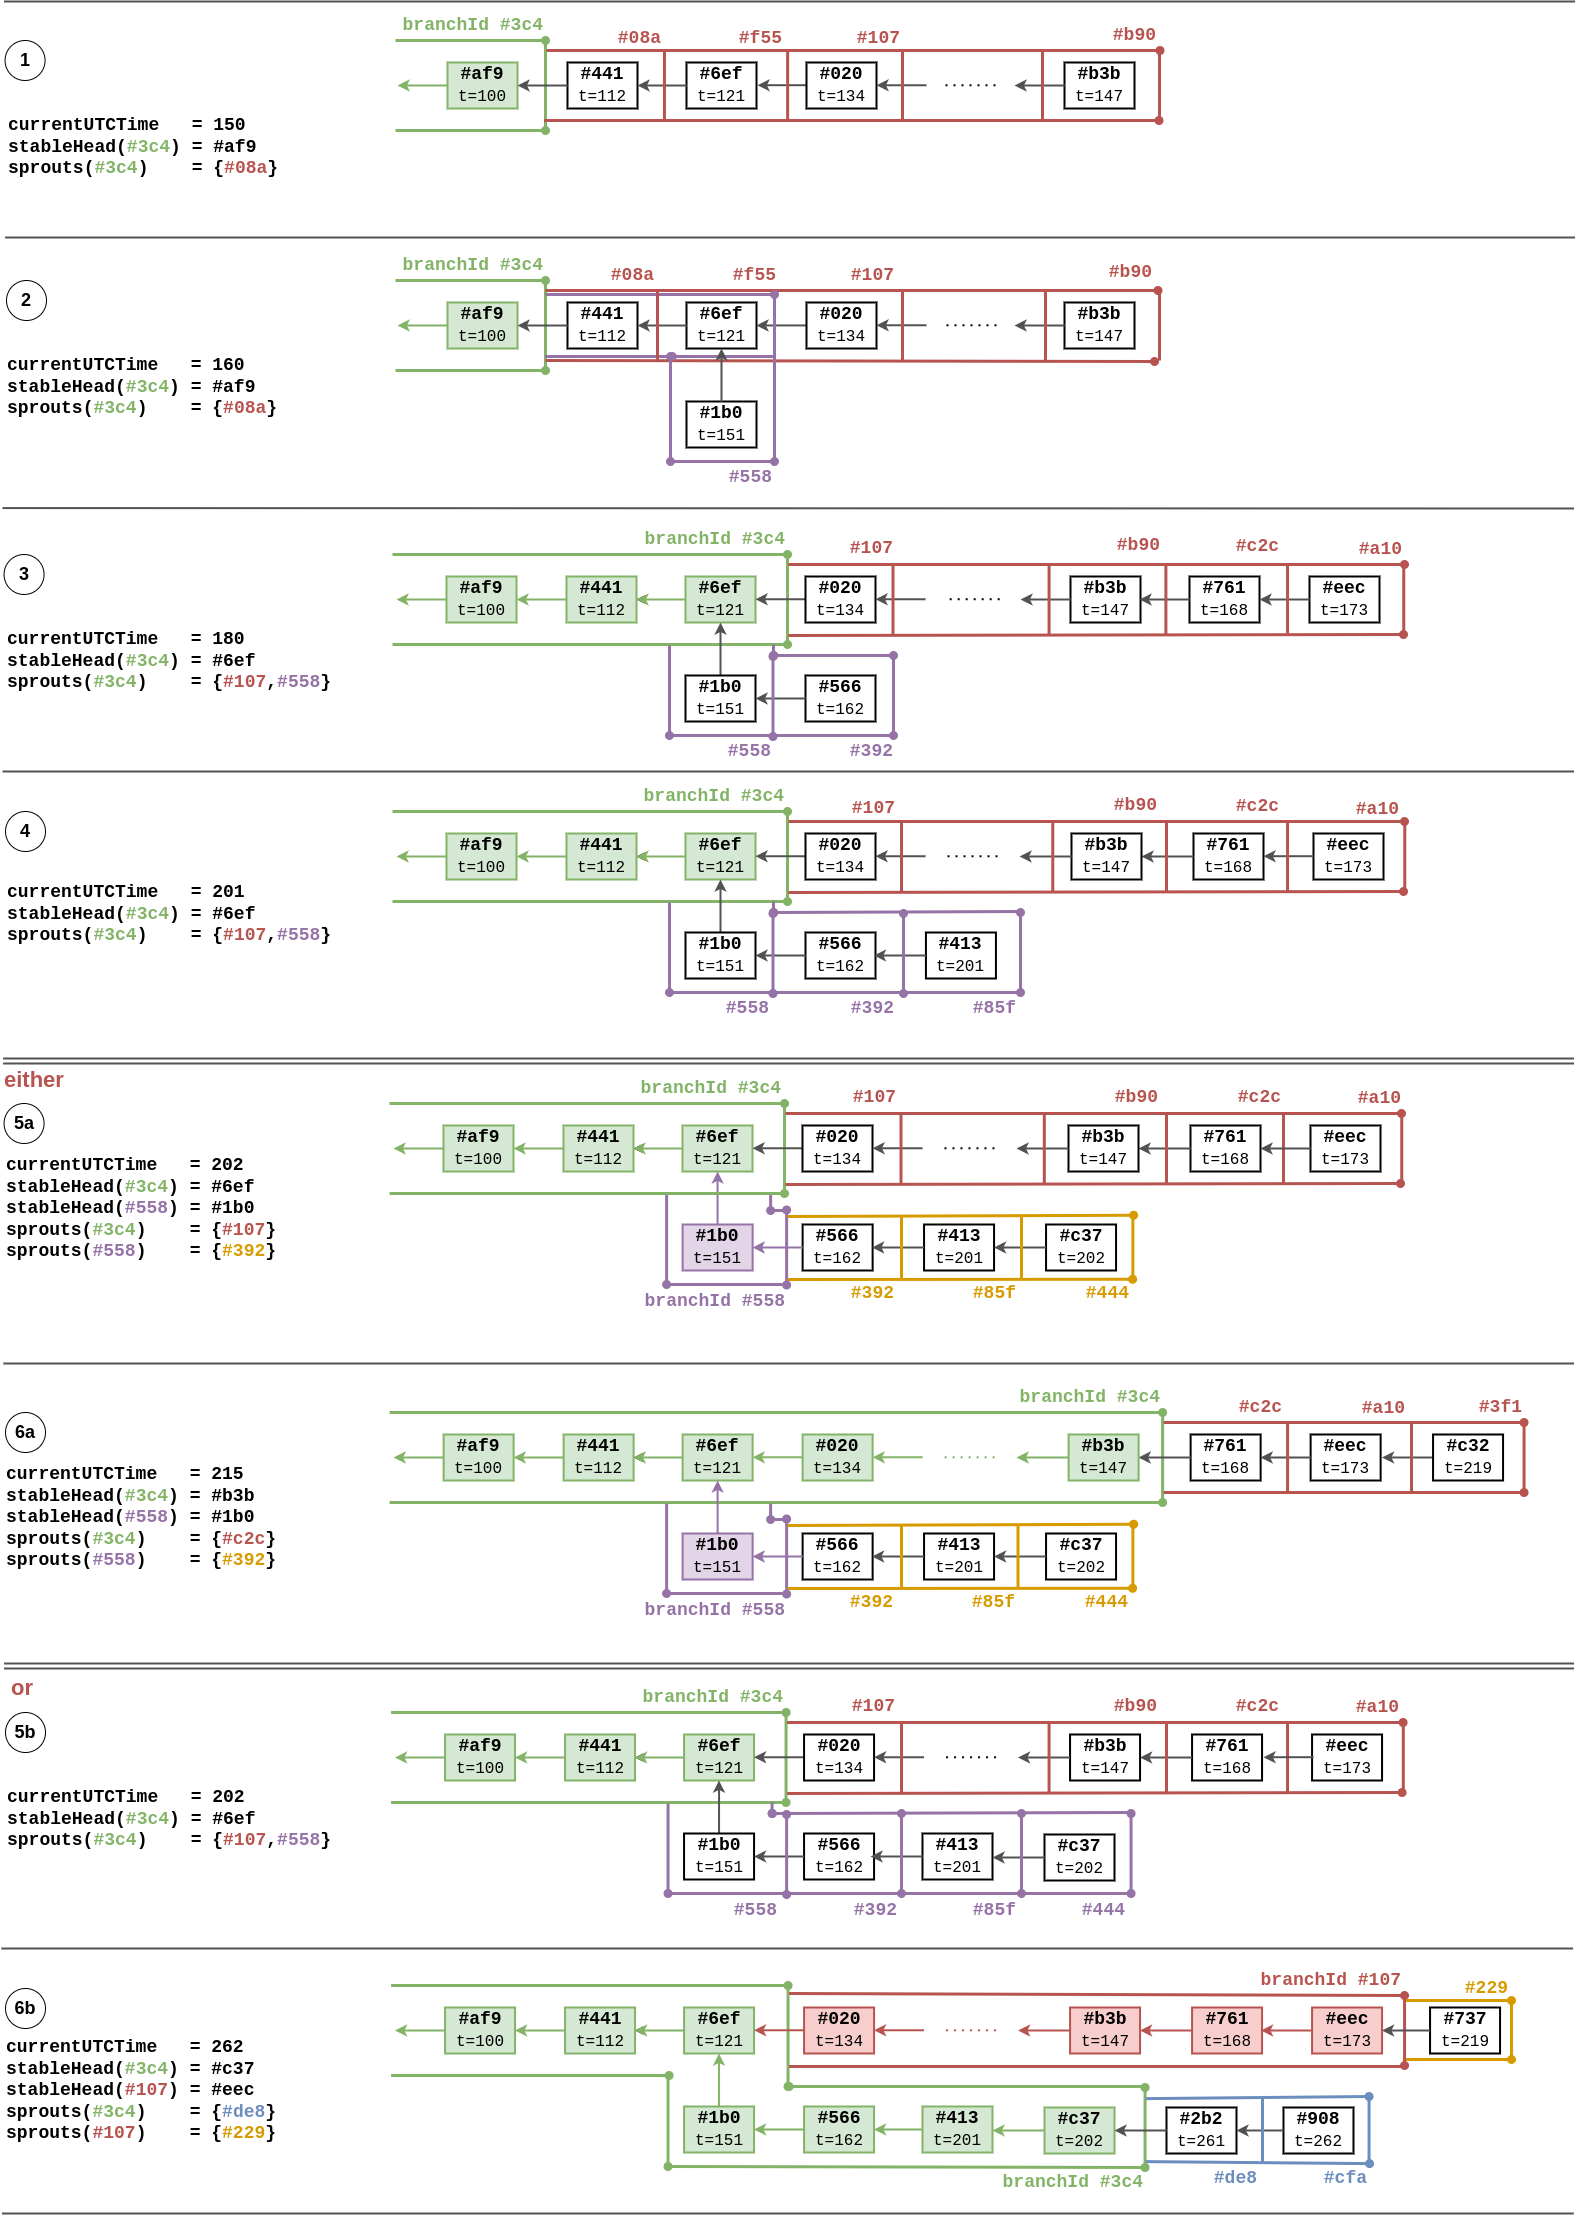
\includegraphics[width=0.82\textwidth]{src/img/LignificationProcessV7.png}
\end{center}
 \caption{Example of a branch lignification with \textit{broadcastingBuffer} $=1$, \textit{lignificationTime} $=50$ and \textit{engagementTime} $=60$. Whenever a new mergeSubmit is added the lignification algorithm \ref{alg:lignification} runs and updates the stable head. The updates 1 to 4 are unambiguous. But then the target branch has two competing sprouts. The default sprout is \textit{\#107} and the other one is \textit{\#558}. Without any veto \textit{\#107} will deliver the next stable head of branch \textit{\#3c4}. This is the scenario 5a. The veto time plus \textit{broadcastingBuffer} have passed and a new mergeSubmit \textit{\#c37} inside sprout \textit{\#444} triggers the lignification algorithm so that the loosing branch \textit{\#558} becomes lignified and rooted in \textit{\#3c4}. In 6a the mergeSubmit lignifies the target branch \textit{\#3c4}. Its head has advanced to \textit{\#b3b}. In scenario 5b a veto had been registered for \textit{\#558} in the sproutSelection entry of the target. If the voting turns out to be in favour of \textit{\#558}, the lignification process will grow the target branch in that direction (c.f. Step 6b).}
 \label{fig:bufferbranches}
\end{figure}


% Comparison to the blockchain case



\subsection{Branch Config Changes}
\label{ssc:configchange}

The branch config contains configurable metadata such as the branch type, a flag that can be set to allow only conflictless submits (see Subsection \ref{ssc:submit}), then the accepted proofs (e.g. proofs of storage, proofs of contributorship,  proofs of token transfer) and also the parameters that determine the consensus (e.g. the number of reviewers needed in the proof of review algorithm). These entries have constrained mutability. They require a merge rather than a plain commit to take effect. For a twig this means that the consensus mechanism for a twig needs to met, i.e. a config-specific fraction of contributors need to approve the merge. For a proper branch this means that the config change needs to go through the proof-of-review (PoR) consensus mechanism (see Subsection \ref{ssc:por}). We envision that in some future release there will be a default schema for the config, but that this schema may be altered through schema buckets to which the schema is pointing.



% \subsubsection{Branch Type Changes}

\subsection{Branch Operations}
\label{ssc:branchops}


\subsubsection*{Creation} 
The first branch operation is the creation. There are \textit{genesis creations} and \textit{rooted creations}. As the name suggest the genesis creation is a branch that does not have ancestorial submits. This is similar to blockchains or git, which have a block or submit without a parent. However unlike those Lakat allows for multiple genesis creations. Anyone can at any time create a new genesis branch, which is either a twig or a proper branch. A genesis creation requires the creator to set the branch config. Optionally the creator may also specify a branch token. 
On the other hand a rooted creation is a branch creation whose initial submit has a parent submit. There are two ways that rooted creations come about. One possibility is that a creator starts a new branch and chooses a parent submit as a root. Anyone may do that for any root branch at any time. The config can then either be chosen anew or inherited. Another possibility involves an ousted sprout, namely one that has been attempting to provide the next stable head in a lignification process. If that ousted sprout receives another submit, it turns into a proper branch. This branch is rooted in the branch for which it was a sprout. It inherits the branch config, but not the token and the branch contributors are the creator of the sprout and the content contributors of the branch that has been attempted to be merged. Any of those contributors can create submits to that ousted sprout and with that submit it turns into a proper branch where the parent entry is set during that conversion. Thus this mechanism for a rooted branch creation is indirect and can only be executed by the respective content contributors.

The creation of branches is permissionless. It is therefore a potential vector for a denial of service attack. The attacker can create a lot of branches and bombard other nodes with branch creation requests. One may leverage the token entry in a newly created branch to mitigate this risk. The attachment of a proof of token transfer in the token entry of the branch can function as a filter for sincere branch creation broadcasts.  

\subsubsection*{Merge}
In Lakat a merge is the inclusion of changes from one branch into another. There is a strict directionality in a Lakat-merge. Git distinguishes between this and other and in Lakat this corresponds to core and peri, where core is the pulling branch. Merging into a proper branch can only occur after a pull-request (see Proof-of-Review in Subsection \ref{ssc:por}). Twigs on the other hand can pull other branches using an approval of a fraction of its content contributors. The fraction is specified in the branch config. After a merge the belt branch may become stale. A stale branch cannot receive submits. Whether a branch becomes stale after a merge depends on the branch config (see Subsection \ref{ssc:configchange}).
A merge requires a merge submit (see Subsection \ref{ssc:submit}) and a cryptographic validation of the branch that is merged. When the conditions for a merge are not met, the merge submit cannot pass the cryptographic validation. For instance if the config of the pulling branch only allows conflictless submits and the belt branch has conflicted submits, then the merge is invalid.

In order to discuss which data buckets are included in the merge submit we briefly introduce the set theoretic slang of $A$ \textit{minus} $B$ for the set of elements in $A$ that are not in $B$. The set of elements that are in $A$ and $B$ is called \textit{intersection} of $A$ and $B$ and the set of elements that are in $A$ or $B$ is called the \textit{union} of $A$ and $B$. The respective notations are $A-B$, $A\cap B$ and $A\cup B$. We denote the set of submits of a branch $\mathfrak B$ by $\mathcal S_{\mathfrak B}$. We denote the set of data buckets in the data root of a submit $s$ by $\mathcal{B}_s$. Thus the set of data buckets in a branch $\mathfrak B$ with stable head $head(\mathfrak B)$ is $\mathcal{B}_{head(\mathfrak B)}$. 

We have already discussed that there is no many-to-one relation between buckets and branches (c.f. Figure \ref{fig:branchbucketrel}). There may be data buckets in core $\mathfrak C$ that are not in belt $\mathfrak P$ and there sure are data buckets in belt that are not in core, i.e. $\mathcal S_{\mathfrak P}-\mathcal S_{\mathfrak C}\neq \emptyset$ is not empty. 
One question that arises in the context of merges is how to combine disparate bucket sets and how to handle that on the level of submits. There are two possible design choices. Either all the submits of belt become submits of core and consequentially also the buckets in $\mathcal S_{\mathfrak P}-\mathcal S_{\mathfrak C}$. Alternatively they stay submits of belt and the beforementioned buckets are included in the merge-submit's merkle hash of the data trie. In the first scenario one is faced with the problem, that the submits of belt all have immutable timestamps and parents. Rebasing those would require to loosen those immutability conditions. In the latter scenario one needs to point to the submits that whose data was included. It suffices to point to the peri's last submit before the merge. We opt for the second scenario. Unlike the first scenario, the second scenario has the peculiar situation that belt may have data buckets in common with core even though they do not share any submits, i.e. $\mathcal S_{\mathfrak P}\cap\mathcal S_{\mathfrak C}= \emptyset$ yet $\mathcal B_{\mathfrak P}\cap\mathcal B_{\mathfrak C}\neq \emptyset$. The only way this can happen in Lakat is if core and belt have pulled from the same branch or from branches that have a common submit in their histories \footnote{Here we make the distinction between the history of a branch and the set of submits of a branch. A branch may be rooted in another branch, but its history can go beyond the root.}. 

% 
% If a merge would include 
% 
% This is a consequence of the way a merge
% 
% The merge submit contains all the buckets of the pulled branch. 
% 
% If the merge follows a pull-request all the content contributors of the requesting branch become also content contributors of the pulling branch.
% 
% 
% password recovery.  ... upon contribution you receive a share


